The Google Glass graphical user interface (GUI) is called a timeline\cite{ImagesGoogleGlassUI} (see Figure \ref{GoogleGlassUI}). The timeline consists of a row of cards. Cards are basic applications such as a clock (see Figure \ref{GoogleGlassCards} (a)) or information about the weather. Cards can also represent more in-depth applications, on Google Glass called ``Immersions'' (see Figure \ref{GoogleGlassCards} (b) and (c)). Immersions handle activities such as browsing an image gallery or playing a game.

	\begin{figure}[ht!]
		\centering
		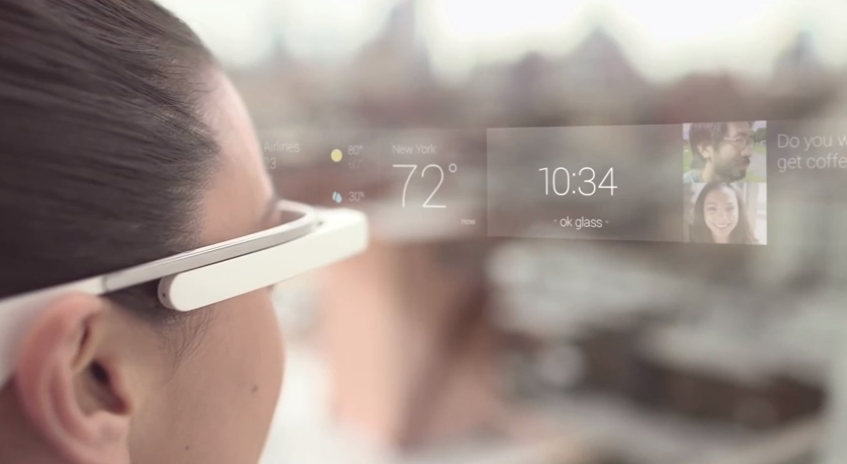
\includegraphics[width=110mm]{images/GoogleGlassUI}
		\caption{A visualisation of the timeline as the timeline is perceived by the user~\cite{ImagesGoogleGlassUI}.}
		\label{GoogleGlassUI}
	\end{figure}

The first screen the user sees when starting up Google Glass is the home screen. The home screen displays a clock and also shows the text "ok glass", as seen in Figure \ref{GoogleGlassCards} (a). The home screen is a part of the timeline and acts as the center point. Cards to the left of the home screen are upcoming activities such as an event in the user's calendar or an upcoming flight. Cards to the right of the home screen are from the past. Cards from the past will for instance show text messages or photos.

	\begin{figure}[ht!]
		\centering
   	\subfloat[The Google Glass home screen is a card that displays a clock.]{{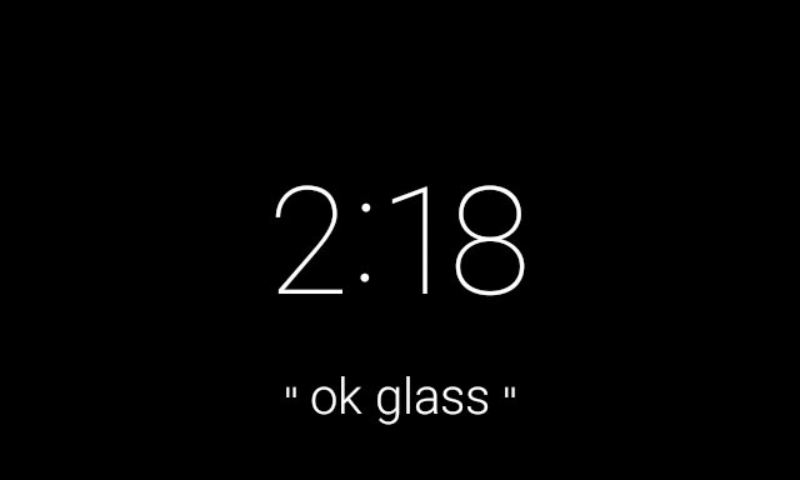
\includegraphics[width=70mm]{images/GoogleGlassHomescreen} }}
  	 \qquad
   	\subfloat[The card ``Explore stars'' represents an immersion.]{{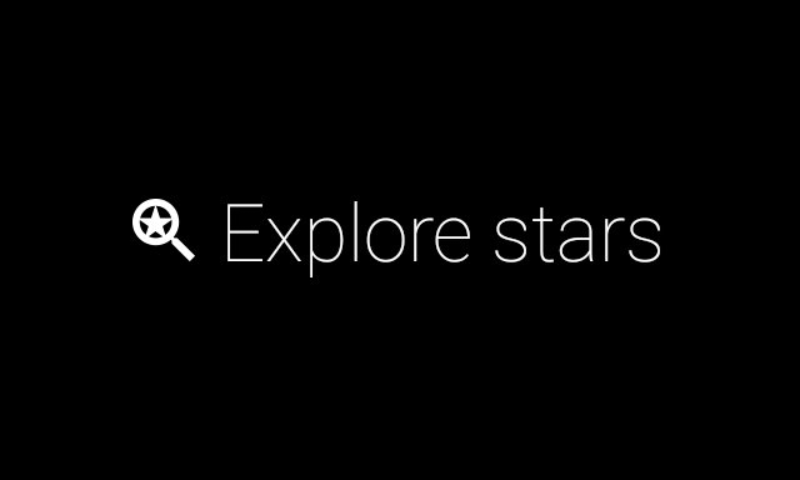
\includegraphics[width=70mm]{images/GoogleGlassStarImmersion} }}
   	\qquad
	\subfloat[The immersion ``Explore stars'' allows the user to look around at stars using the built-in head motion tracker.]{{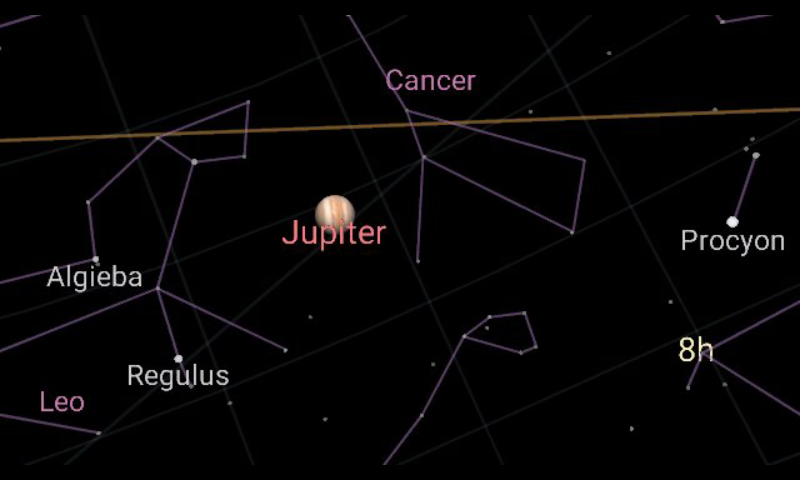
\includegraphics[width=70mm]{images/GoogleGlassStarImmersion2} }}
   	\qquad
		\caption{Cards can either display basic applications or represent immersions.}
		\label{GoogleGlassCards}
	\end{figure}

In order to move left on the timeline (forward in time) the user must swipe a finger backwards on the touchpad. In order to move right on the timeline (backward in time) the user must swipe a finger forward on the touchpad. The fact that the user must swipe backwards when stepping forward in time might not seem especially intuitive. In western culture a timeline is normally represented as going from left to right. One example is books, where the reader not only reads each line from left to right, but also turn pages from the right (the future) to the left (the past). However, on Google Glass, the swiping action could be thought of as swiping cards behind the back. Swiping forward when stepping backwards in time would then in turn mean bringing cards placed behind the back into focus. Cards in the past are behind the user while cards in the future are in front of the user.

When the user wants to turn off Google Glass the user swipes down on the touchpad. Swiping down on the touchpad will put Google Glass in stand-by mode. If the user wants to turn off Google Glass entirely, in other words power down the device, there is a power button on the opposite side of the touchpad. Holding down the power button for a few seconds will turn off Google Glass. For a better visual understanding of how Google Glass works see Figure \ref{GoogleGlassUI} as well as the video referenced in the caption.

Google Glass uses a Bone Conduction Transducer (BCT) to transfer sound to the user~\cite{GlassSpecs}. The BCT transfers sound to the inner ear by conducting sound through the bones of the skull~\cite{boneConductionWiki}. The advantage of this technique is that the sound maintains clarity, even in noisy environments. Also, since the user does not plug any earphone into their ears, external sound is not blocked out.

Google Glass also features a 5 megapixels camera. The camera sits between the touchpad and the display, as seen in Figure \ref{GoogleGlassHardware} (b), and is capable of capturing video at a 720p resolution. The camera can be used for video conferencing, as Google showed in 2012~\cite{glassLiveDemo}, but the camera can for instance also be used when the user wants to scan a QR Code\footnote{See section \ref{subsec:qrcode}}.

The user can also interact with Google Glass using voice commands. As seen in Figure \ref{GoogleGlassCards} the home screen consists not only of a clock but also of the words ``ok glass'', in quotes. ``ok glass'' indicates to the user that voice commands are available. The voice command menu is accessed as soon as the user says the words ``ok glass''. Doing so brings up a list of voice commands available, as seen in Figure \ref{voiceCommandMenu}.

	\begin{figure}[ht!]
		\centering
		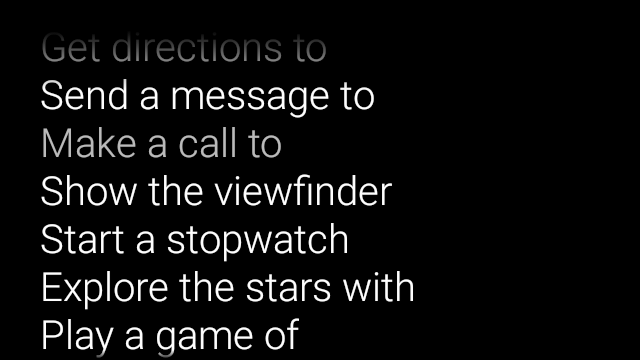
\includegraphics[width=110mm]{images/glassVoiceMenu}
		\caption{Saying ``ok glass'' will bring up the voice vommand menu. \cite{googleGlassVoiceCommand}}
		\label{voiceCommandMenu}
	\end{figure}

In order to progress further the user must say one of the options being displayed out loud. Doing so will either make Google Glass perform the task spoken or give the user the option to add an input option to the task chosen. For instance, if the user where to say ``ok glass, Start a stopwatch'', Google Glass would start a stopwatch.

Google Glass also supports head motions as a form of input from the user. Head motions are not enabled in the timeline as a way of input but tilting the head may wake up Google Glass from stand by mode, if the user has enabled the head wake up feature~\cite{headWakeUp}. The head motion interface may also be used in certain immersions, such as ``Explore stars'' seen in Figure \ref{GoogleGlassCards} (c).
%The main way for a user to give input to Google Glass is via the touchpanel that is mounted on the right hand side of Glass, along the frame. Users are able to swipe as well as tap, which gives them control similar to that of a Smart TV's user interface. Where with a TV controller the user would maneuver with a simple cross layout (up, down, right and left) the buttons have on Glass been replaced by a touchpanel.\\

% Insert image of Google Glass graphical user interface here!!!

%The graphical interface is displayed at the top right through a projection coming from the right on a thick piece of glass. This technique lines up the image with the users sight but does not give any projection outwards.\\

%The interface is built with cards. Each card represents an activity.\\

%What’s unique?
%Standards?
%\url{https://developers.google.com/glass/design/}